\documentclass{paper}

%\usepackage{times}
\usepackage{epsfig}
\usepackage{graphicx}
\usepackage{amsmath}
\usepackage{amssymb}
\usepackage{color}


% load package with ``framed'' and ``numbered'' option.
%\usepackage[framed,numbered,autolinebreaks,useliterate]{mcode}

% something NOT relevant to the usage of the package.
\setlength{\parindent}{0pt}
\setlength{\parskip}{18pt}






\usepackage[utf8]{inputenc} 

\usepackage{listings} 
\lstset{% 
   language=Python, 
   basicstyle=\small\ttfamily, 
} 



\title{Photometric stereo}



\author{Aaron Karper\\08-915-894}
% //////////////////////////////////////////////////


\begin{document}



\maketitle


% Add figures:
%\begin{figure}[t]
%%\begin{center}
%\quad\quad   \includegraphics[width=1\linewidth]{ass2}
%%\end{center}
%
%\label{fig:performance}
%\end{figure}

\section{Photometric Stereo (Due on 29/10/2013)}

\subsection{Calibration (35 points)}
First step was finding the specular reflection of the light source in the image. I solved this by first blurring the image with a Gaussian kernel and then finding the maximum intensity pixel. The rationale is that there may be many pixels at maximum intensity 255, but with the blurring only a few remain (basically this is similar to an erode filter), which should give a reasonable approximation of the light source in the image.

The next step is finding the radius and the center of the sphere, which can be calculated simply by taking the terms of the mask in x and y direction and taking the number of non-zero ones divided by 2 for the radius. I also added averaging of the calculation in x and y direction because I'd hate to see perfectly valid information going to waste.\\
For the center, we can calculate the mean of the indices of the non-zero terms, which gives us $(c_x, c_y)$.

To get the $z$ coordinate of the sphere normal, we now use
\[ z^2+(y-c_y)^2+(x-c_x)-^2 = r^2 \Rightarrow z = \sqrt{r^2-(y-c_y)^2-(x-c_x)^2}\]
which sets the origin of $z$ to the center of the sphere.

We can conclude that the light $l$ and its reflection on the sphere $l'$ fulfil
\begin{align*}
l&\propto 2\,\mathbf{n}\cdot \mathbf{l}\, \mathbf{n} - l'
\end{align*}
\begin{center}
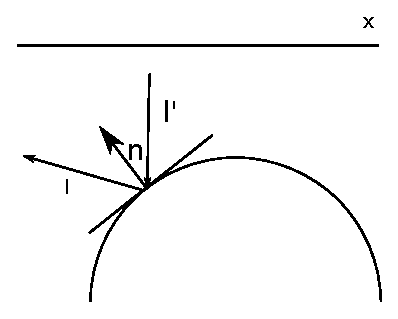
\includegraphics[width=0.5\linewidth]{out/reflection.pdf}
\end{center}
\begin{itemize}
\item The so calculated directions don't seem to be terribly wrong, but they don't seem to be terribly right either. I suspect a bug in the code somewhere. The following sections use the example lights instead.

\begin{align}
\mathbf{L}^T= \left[ \begin{array}{ccc}
-0.246&0.267&-0.932\\
-0.071&0.125&-0.990\\
-0.088&-0.017&-0.996\\
-0.221&-0.050&-0.974\\
-0.263&-0.167&-0.950\\
-0.296&-0.050&-0.954\\
-0.213&0.142&-0.967\\
-0.221&0.058&-0.973\\
-0.171&0.109&-0.979\\
-0.171&0.050&-0.984\\
-0.021&0.067&-0.998\\
-0.180&-0.067&-0.981
\end{array} \right] \nonumber
\end{align}
\end{itemize}


\subsection{Computing Surface Normals and Grey Albedo (30 points)}
This relies on the fact that the normal gives the direction, but the albedo gives the magnitude of the $\tilde{n}_{xy}$ vectors.

The interesting step is now to find the $\tilde{n}_{xy}$: Our model tells us that the intensity is $I_i=\mathbf{l_i}\cdot \mathbf{\tilde{n}}$ in every image, or $\mathbf{I}=L\,\mathbf{\tilde{n}}$ for all images. We constructed $L$ in the previous step and can now solve (least square) for $\mathbf{\tilde{n}}$ by reshaping the image into a vector of RGB intensities, solving the least square problem and reshaping the solution back into the original dimension (plus the directions). At this point I defer the ``greying" of the image until after the calculation of the normals -- I calculate the normals for each channel and take the mean of the normals.
\begin{lstlisting}[language=Python]
images.shape = (nimages, -1,)
normals = least_square(lights, images)[0]
normals.shape = (3, width, height, colors)
\end{lstlisting}

\subsubsection{Results}
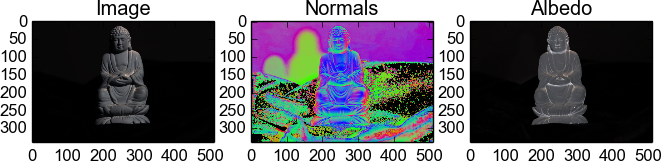
\includegraphics[width=1\linewidth]{out/buddha_normals.png}
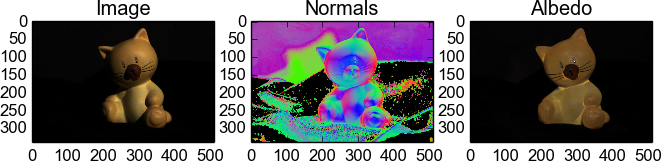
\includegraphics[width=1\linewidth]{out/cat_normals.png}
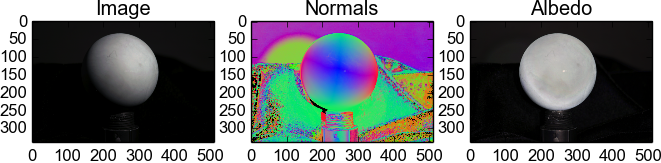
\includegraphics[width=1\linewidth]{out/gray_normals.png}
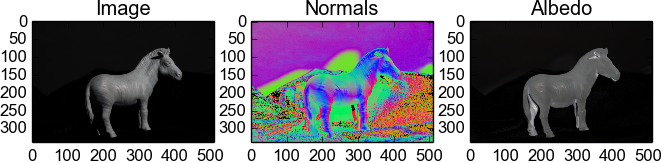
\includegraphics[width=1\linewidth]{out/horse_normals.png}
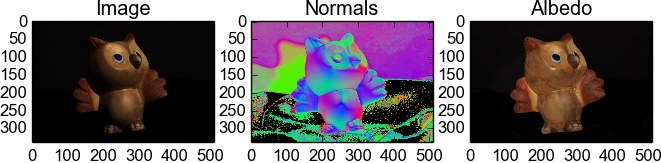
\includegraphics[width=1\linewidth]{out/owl_normals.png}
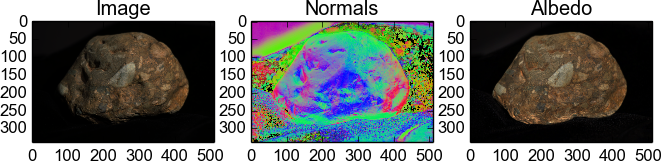
\includegraphics[width=1\linewidth]{out/rock_normals.png}

To calculate the normals, I take the channelwise mean of $\tilde{n}$ and divide by their length. For the albedo, I take the length of the $\tilde{n}$s and normalize them into $[0,1]$

\subsection{Surface Fitting (35 points)}

The fitting of the surface is again a least square problem, the challenge is constructing the system and reconstructing the solution. For this I use a bimap from $(x,y)$ coordinates to rows in the system I want to generate, dropping every pixel not on the mask.

For every pixel that is on the mask I add two rows to the system so that the pixel has a weight of $1$ and in the first row its $x$-neighbour and the second row its $y$-neighbour have a weight of $-1$. The $b$ to be solved for has $\frac{n_x}{n_z}$ and $\frac{n_y}{n_z}$ respectively in these rows. This models the fact that $\frac{\partial z}{\partial x}\cdot n =\frac{\partial z}{\partial y}\cdot n = 0$ by approximating the derivative with the finite difference of the adjacent pixels\footnote{A more robust way might be to take a more elaborate approximation taking more neighbours into account.}.

A refinement I tried, but which gave worse result, was introducing the constraint that the edge pixels should be approximately 0.

\subsubsection{Results}
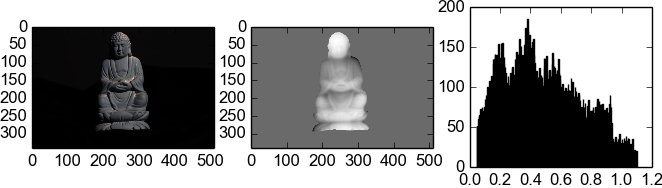
\includegraphics[width=1\linewidth]{out/buddha_depth.png}
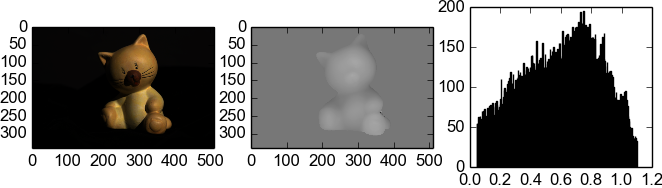
\includegraphics[width=1\linewidth]{out/cat_depth.png}
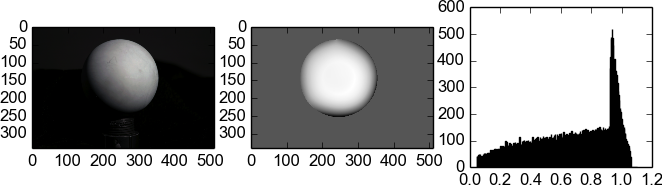
\includegraphics[width=1\linewidth]{out/gray_depth.png}
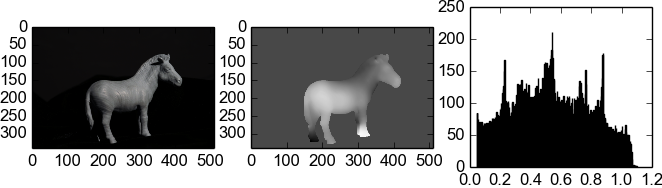
\includegraphics[width=1\linewidth]{out/horse_depth.png}
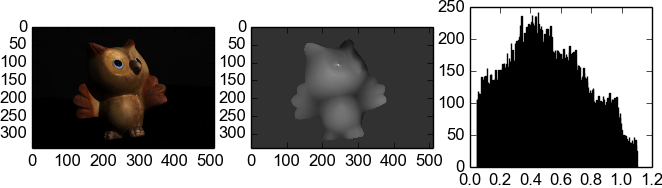
\includegraphics[width=1\linewidth]{out/owl_depth.png}
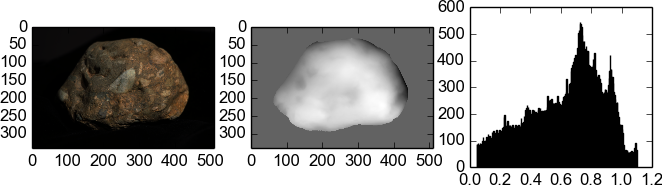
\includegraphics[width=1\linewidth]{out/rock_depth.png}

Two obvious mistakes are on the buddha model (head is too far to the front) and the horse model (hoof on the right is too far to the front).

In the horse suffers from the fact that the front left hoof is often badly illuminated and thus has a bad approximation of the normals. This leads to the locally bad approximation of the depth of the hoof.

The Buddha model suffers from a similar problem, because the bottom left corner of the face casts a shadow and gives bad normals, which translate to a bad depth.

Both are caused by cast shadows, which are not part of our model. If it was possible to take this into account when calculating the normals, e.g. by discarding the information of suspicious pixels, I could probably get rid of these artefacts.
 \end{document}